\documentclass[12pt]{article}
%\usepackage[spanish]{babel} 
\usepackage[utf8]{inputenc}
\usepackage{tgheros}
\renewcommand{\familydefault}{\sfdefault}
\usepackage{authblk}
\usepackage{setspace}
\usepackage[margin=1.25in]{geometry}
\usepackage{graphicx}
\graphicspath{ {./figures/} }
\usepackage{subcaption}
\usepackage{blindtext}
\usepackage{hyperref}
\usepackage{bookmark}


% Cargar apacite después de babel para citas autor-año correctas
\usepackage[notocbib]{apacite} 

% other packages
\usepackage{latexsym,amsmath,xcolor,multicol,booktabs,calligra, tcolorbox}
\usepackage{graphicx,listings,stackengine}
% Manejo robusto de nombres de archivo con espacios y rutas de imágenes
\usepackage{grffile}

% Keywords command
\providecommand{\keywords}[1]
{
  \small	
  \textbf{\textit{Keywords---}} #1
}

\title{Modelamiento de Lahares Mediante Redes Neuronales Informadas por la Física (PINNs): Aplicacion al Evento Eruptivo de 2015 del Volcán Villarica, Chile}

\author[1]{Dylan Jara Carvajal}
\author[2]{Felipe Herrera (Profesor Guía)}
\author[3]{Johan Triana (Profesor Co-guía)}
\author[4]{Yuvineza Gomez-Leyton (Profesor informante)}
\author[5]{Francisco Plaza-Vega (Profesor informante)}

\affil[1,2,5]{Departamento de Matemática y Ciencia de la Computación\\Universidad de Santiago de Chile}
\affil[3,4]{Departamento de Física\\Universidad Católica del Norte}

\date{\today}
\onehalfspacing
\begin{document}
\maketitle
  
\begin{abstract}
    Se realizó un acople entre una Physics-Informed Neural Network (PINN) y un sistema de ecuaciones diferenciales parciales para la predicción de la morfodinámica de un lahar producido por un evento eruptivo del 2015 del volcán Villarica, Chile.   
\end{abstract}
\keywords{Physics-Informed Neural Network, Lahares, Ecuaciones Diferenciales Parciales}

\section{Objetivos de la Tesis}
\subsection{Objetivo General}
Desarrollar un modelo de lahares basado en redes neuronales informadas por la física (PINNs), aplicado al evento eruptivo de 2015 del volcán Villarica, Chile, incorporando ecuaciones acopladas de flujo somero, concentración sólida y presión de poros.
\subsection{Objetivos Específicos}
\begin{enumerate}
    \item Formar un sistema de ecuaciones compuesto con, al menos, seis ecuaciones diferenciales parciales que modelen la morfodinámica de un lahar en el evento eruptivo del año 2015 del volcán Villarica, Chile.
    \item Construir una red neuronal informada por la física usando el sistema de PDEs y otros parámetros geológicos que prediga el comportamiento real de un flujo de sedimento. 
    \item Diagnosticar patologías de desvanecimiento y decaimiento de los gradientes e incorporar técnicas de estabilización y optimización avanzadas para mejorar la convergencia del modelo.
    \item Predecir la morfodinámica de manera realista y acorde a la física para exportar un mapa de peligro volcánico que entregue datos de evacuación según el riesgo calculado por la red neuronal.   
\end{enumerate}

\newpage
\section{Carta Gantt}
\begin{table}[htbp]
\centering
\caption{Planificación de Actividades del Trabajo de Título (Marzo 2026 - Marzo 2027)}
\label{tab:planificacion_gantt}
\renewcommand{\arraystretch}{1.3} % Da un poco más de espacio entre las filas
\begin{tabular}{|c|p{7cm}|c|c|c|}
\hline
\textbf{ID} & \textbf{Actividad} & \textbf{Inicio} & \textbf{Término} & \textbf{Objetivo(s)} \\ \hline
1 & Revisión bibliográfica de PINNs y reología de lahares & 02/03/2026 & 31/03/2026 & OE1 \\ \hline
2 & Definición y adimensionalización del sistema de PDEs & 01/04/2026 & 30/04/2026 & OE1 \\ \hline
3 & Programación del módulo de topografía y lecho seco & 04/05/2026 & 22/05/2026 & OE2 \\ \hline
4 & Implementación del \textit{Ansatz} (Hard Constraints) para IC & 25/05/2026 & 12/06/2026 & OE2 \\ \hline
5 & Obtencion de predicciones en el orden de 10e-3 & 15/06/2026 & 03/07/2026 & OE2 \\ \hline
6 & Configuración de normalización y callbacks & 06/07/2026 & 31/07/2026 & OE3 \\ \hline
7 & Redacción de Capítulos 1 (Intro) y 2 (Marco Teórico) & 03/08/2026 & 21/08/2026 & Doc. \\ \hline
8 & Ejecución Etapa 1: Ajuste de IC/BC y masa inicial & 24/08/2026 & 11/09/2026 & OE3 \\ \hline
9 & Ejecución Etapa 2: Entrenamiento de Masa y Momento & 14/09/2026 & 09/10/2026 & OE3 \\ \hline
10 & Ejecución Etapa 3: Acople de Concentración y Presión & 12/10/2026 & 06/11/2026 & OE3 \\ \hline
\end{tabular}
\end{table}
\clearpage

\begin{table}[htbp]
\centering
\caption{Planificación de Actividades del Trabajo de Título Parte 2(Marzo 2026 - Marzo 2027)}
\label{tab:planificacion_gantt}
\renewcommand{\arraystretch}{1.3} % Da un poco más de espacio entre las filas
\begin{tabular}{|c|p{7cm}|c|c|c|}
\hline
\textbf{ID} & \textbf{Actividad} & \textbf{Inicio} & \textbf{Término} & \textbf{Objetivo(s)} \\ \hline
11 & Implementación de técnicas para Trivial Solution Collapse & 09/11/2026 & 27/11/2026 & OE4 \\ \hline
12 & Optimización final con L-BFGS y Learning Rate Decay & 30/11/2026 & 24/12/2026 & OE3 \\ \hline
13 & Redacción de Capítulo 3 (Metodología) & 28/12/2026 & 15/01/2027 & Doc. \\ \hline
14 & Pruebas de sensibilidad y cuantificación de error & 18/01/2027 & 05/02/2027 & OE4 \\ \hline
15 & Validación vs. Modelos Numéricos Tradicionales & 08/02/2027 & 26/02/2027 & OE4 \\ \hline
16 & Análisis de resultados y generación de visualizaciones & 01/03/2027 & 12/03/2027 & OE4 \\ \hline
17 & Redacción de Capítulos 4 (Resultados) y 5 (Conclusiones) & 15/03/2027 & 24/03/2027 & Doc. \\ \hline
18 & Revisión final de formato, citas y bibliografía & 25/03/2027 & 29/03/2027 & Doc. \\ \hline
19 & Preparación de material para defensa de tesis & 30/03/2027 & 30/03/2027 & Examen \\ \hline
20 & Entrega final y cierre de proceso & 31/03/2027 & 31/03/2027 & Hito Final \\ \hline
\end{tabular}
\end{table}

\newpage
\begin{figure}[h!]
    \centering
    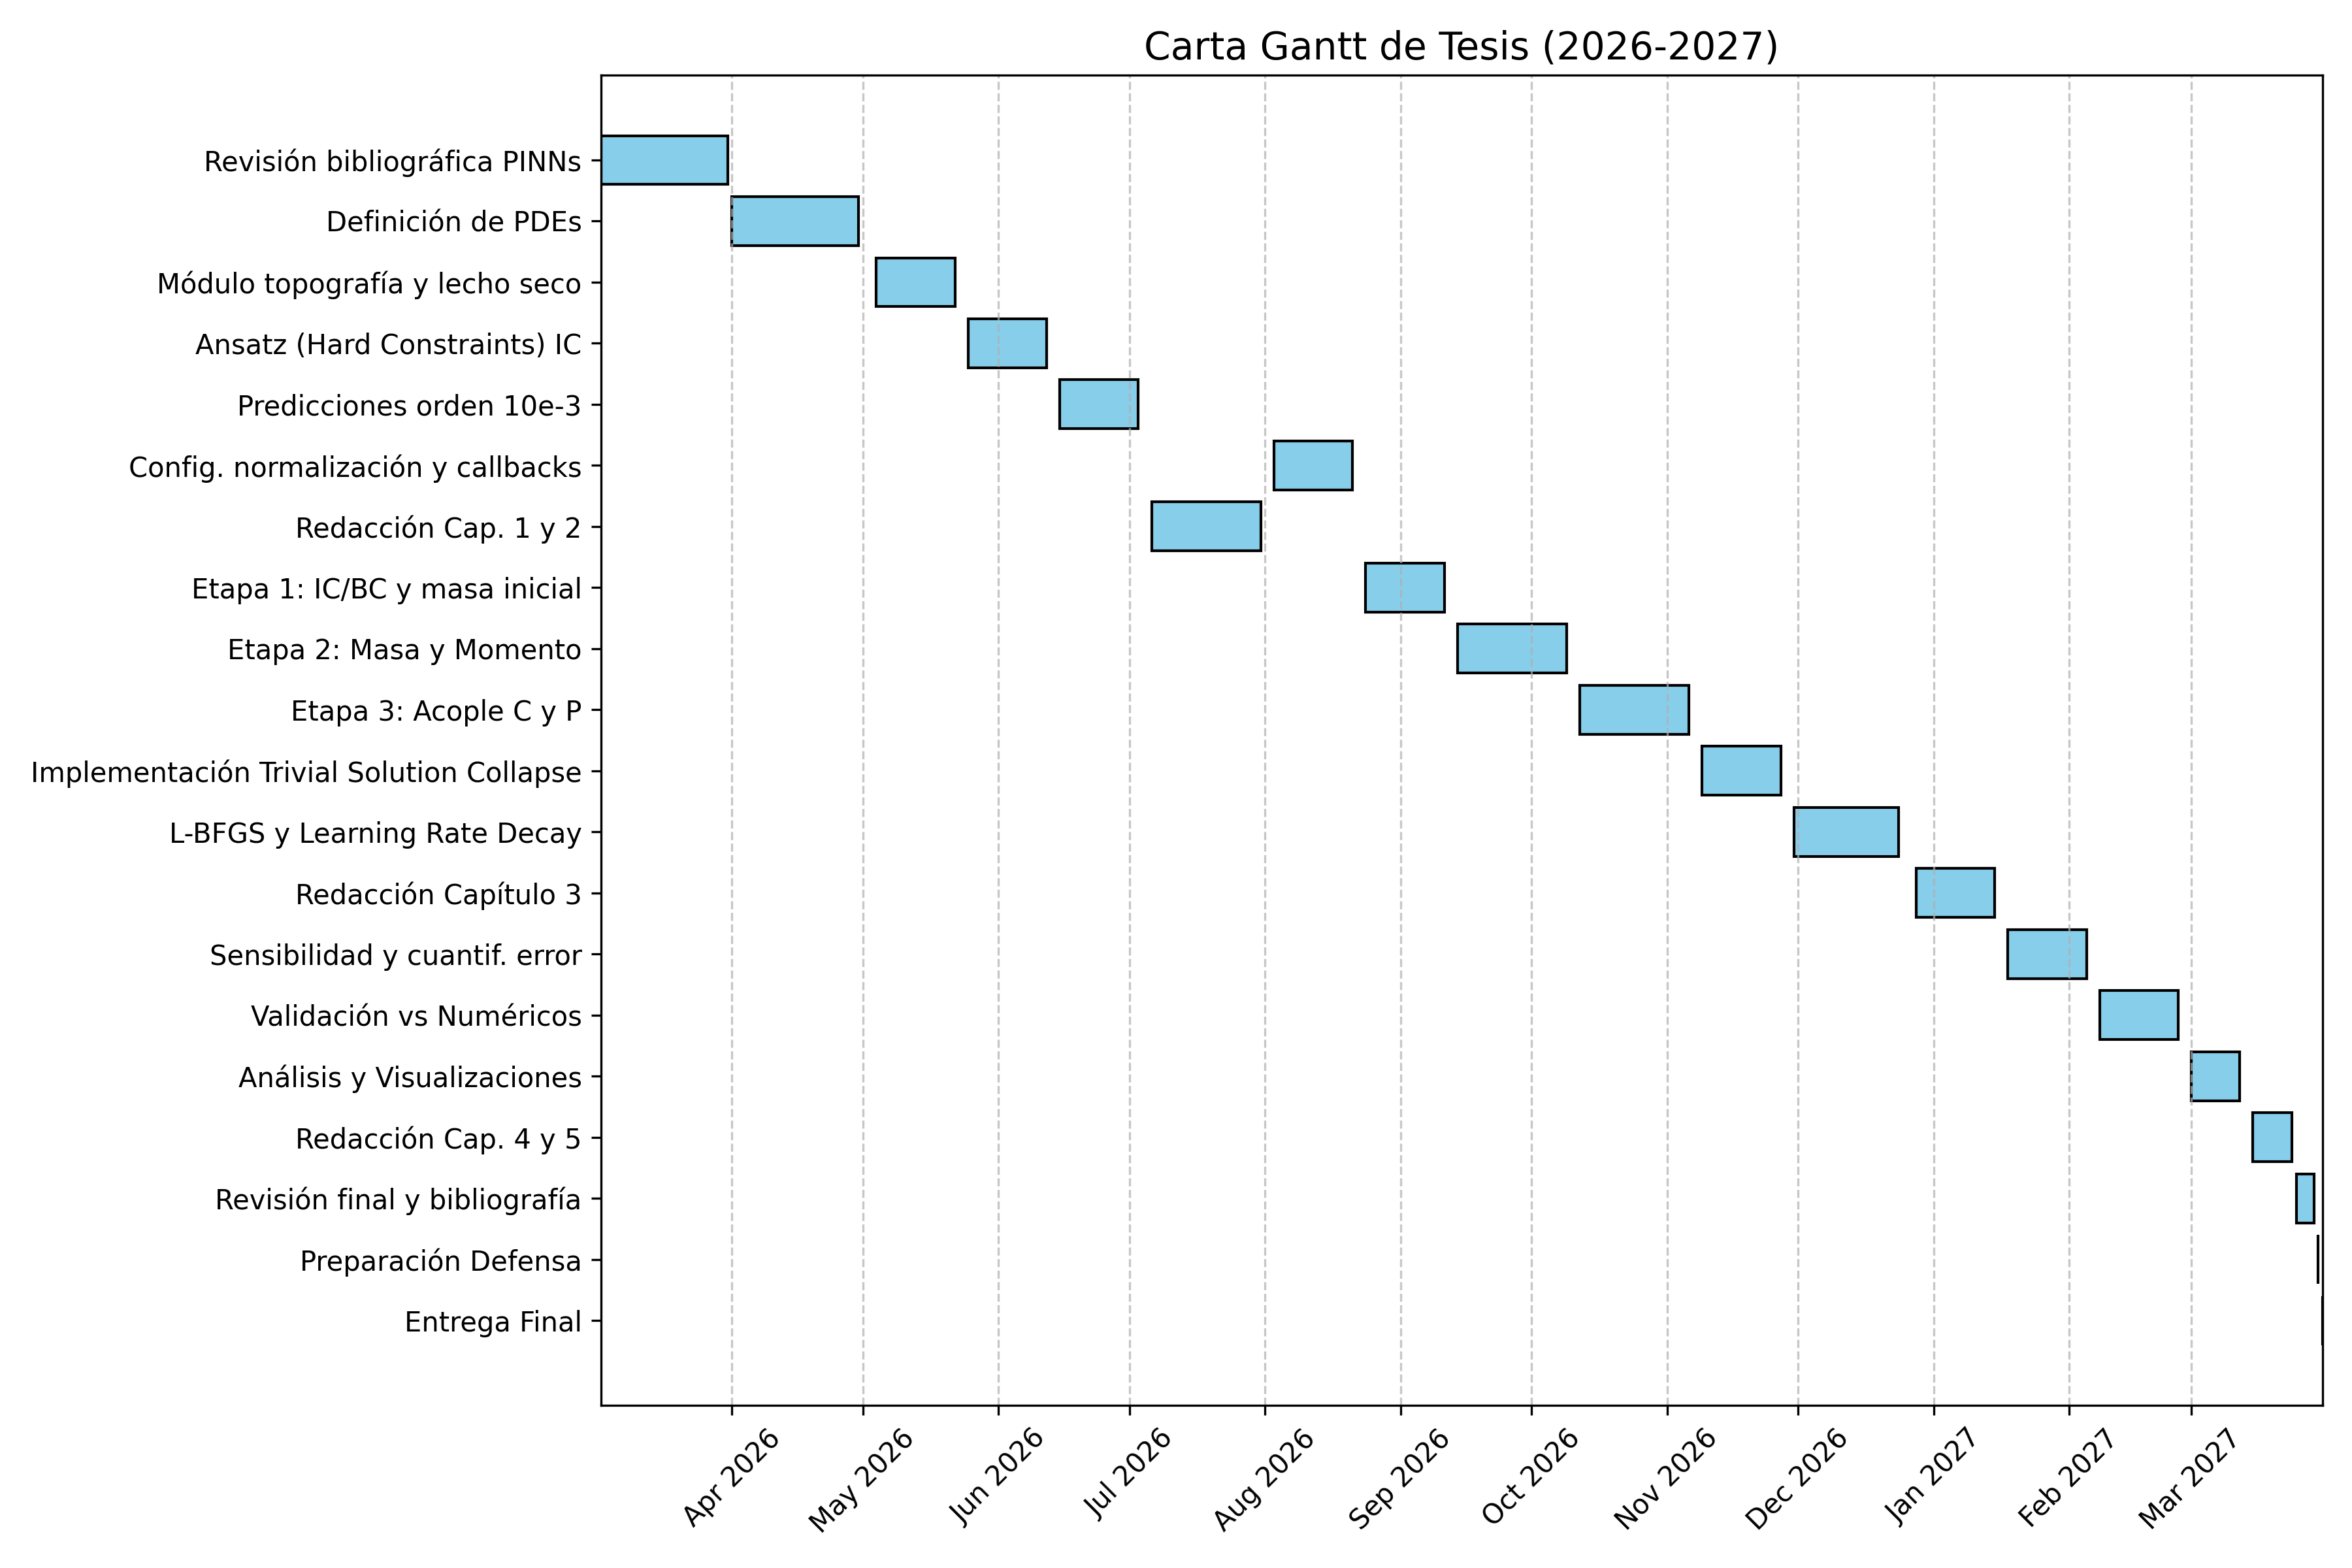
\includegraphics[width=\linewidth]{carta_gantt_tesis.png}
    \caption{Carta Gantt de actividades para el desarrollo del trabajo de título.}
    \label{fig:gantt}
\end{figure}
\nocite{*} % Esto evita el error "no \citation commands" al incluir todo el .bib
\bibliographystyle{apacite} % O "plain", pero apacite es mejor para ciencias
\bibliography{bibliography} % Asegúrate de que el archivo se llame referencias.bib

\end{document}